% !TEX root = ../Thesis.tex
%%
%%  Hochschule für Technik und Wirtschaft Berlin --  Projektabschlussbericht
%%
%% Kapitel 3 - Grundlagen
%%
%%

\chapter{Grundlagen} \label{Grundlagen}
\section{LoRa und LoRaWAN} \label{LoRa und LoRaWAN}
\subsection{LoRa} \label{LoRa}

Der Begriff LoRa steht für \textbf{L}ong \textbf{R}ange und definiert dabei ein für weite Strecken ausgelegtes, funkbasiertes Übertragungsverfahren auf der Bitübertragungsschicht (physical layer) im OSI-Schichtenmodell. Es wurde von Nicolas Sornin und Olivier Seller in deren französischen Firma Cycleo, welche später von Semtech Corporation abgekauft wurde, im Jahr 2009 entwickelt \cite{semtech2020}. 

LoRa kann zu den sogenannten \textbf{L}ow-\textbf{P}ower-\textbf{W}ide-\textbf{A}rea-\textbf{N}etwork (LPWAN) Technologien zugeordnet werden, die einen energiesparsamen Betrieb und eine hohe Übertragunsreichweite aufweisen. Im Vergleich zu WLAN oder Mobilfunk, fällt jedoch die Daten- bzw. Bandbreite bei diesen Technologien relativ gering aus, sodass diese hauptsächlich bei drahtlosen Sensornetzwerken Anwendung finden, wo es darum geht Sensordaten mit einer geringen Datenrate über eine weite Funkstrecke zu übertragen. Ein Vergleich zu den funkbasierten Technologien (WLAN, LPWAN und Mobilfunk) stellt die Abb. \ref{fig:lpwan} dar.

\begin{figure}[h]
 \centering
 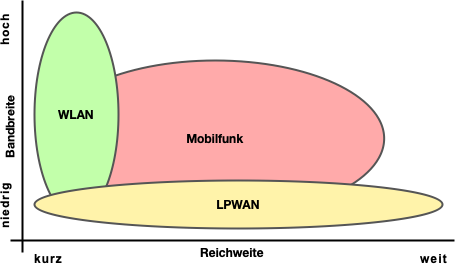
\includegraphics[width=0.7\textwidth]{pictures/lpwan-wlan-mobilfunk}
 \caption[Vergleich zwischen WLAN, Mobilfunk und LPWAN bezüglich der Bandbreite und Reichweite]{Vergleich zwischen WLAN, Mobilfunk und LPWAN bezüglich der Bandbreite und Reichweite \cite{lpwan2022}}
 \label{fig:lpwan}
\end{figure}

Die hohe Reichweite, bei gleichzeitig energiesparsamem Betrieb, erzielen die LPWAN Technologien mithilfe von Frequenzen unterhalb des 1 GHz Bereiches. Da LoRa ebenfalls zu den LPWAN Technologien zählt, nutzt diese in Europa die lizenfreien 433 und 868 MHz ISM-Frequenzbänder. Die Frequenzbänder unterscheiden sich jenach Land und Region auf der ganzen Welt. In den USA z.B. liegt der nutzbare Frequenzband bei 915 MHz. Das 433 MHz Frequenzband ist jedoch nur für unidirektionale Übertragung, wo man entweder nur Senden oder Empfangen kann, vorgesehen. Hingegen ist das 868 MHz Band bidirektional, das heißt, dass damit das gleichzeitige Senden und Empfangen gewährleistet ist \cite{lpwan2022}. 

Die jeweiligen Frequenzbänder haben eine bestimmte Frequenzbandbreite und werden wiederum in sogenannte Funkkanäle unterteilt, mit einer bestimmten Kanalbandbreite, um das gegenseitige stören gleicher Frequenzen zu minimieren. So weist z.B. das 868 MHz Frequenzband eine Frequenzbandbreite zwischen 863 und 870 MHz auf \cite{Staniec2020}. So können benachbarte Funkknoten, die sich im gleichen 868 MHz Frequenzband befinden, aber einen unterschiedlichen Funkkanal nutzen, gleichzeitig senden und empfangen, ohne sich dabei zu stören. 

Darüberhinaus werden weitere regulatorische Maßnahmen ergriffen, wie die Festlegung einer Zeit in Form eines \textbf{D}uty-\textbf{C}ycles (DC), welches angibt, wie lange ein Funkknoten auf das Medium pro Tag zugreifen darf. Dieser ist ein prozentualer Wert und liegt bei LoRa normalerweise bei 1\% oder 10\% je nach Funkkanal und Sendeleistung \cite{Staniec2020}. 

Die Abbildung \ref{fig:868-band} zeigt das 868 MHz-Frequenzband mit den jeweiligen Funkkanälen, deren Bandbreite (in kHz), der äquivalenten Strahlungsleistung (in dBm) und des jeweiligen Duty Cycles an . 

\begin{figure}[h]
 \centering
 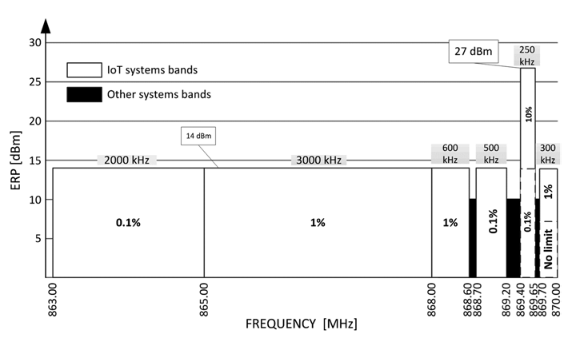
\includegraphics[width=0.9\textwidth]{pictures/868-band}
 \caption[Aufteilung des 868-ISM-Bandes in Funkkanäle nach ETSI EN 300 220-2]{Aufteilung des 868-ISM-Bandes in Funkkanäle nach ETSI EN 300 220-2 \cite{Staniec2020}}
 \label{fig:868-band}
\end{figure}

Weitere Möglichkeiten zur Verhinderung der gegenseitigen Störung, sind die definierten Zugriffsverfahren auf das Medium, die bei LPWAN auch als \textbf{P}olite-\textbf{M}edium-\textbf{A}ccess (PMA) heißen. Darunter zählt das sogenannte \textbf{C}lear-\textbf{C}hannel-\textbf{A}ssessment (CCA), welches wiederum in \textbf{A}daptive-\textbf{F}requency-\textbf{A}gility (AFA) und \textbf{L}isten-\textbf{B}efore-\textbf{T}alk (LBT) eingeteilt werden kann. Dabei ähnelt das CCA-Zugriffsverfahren sehr stark dem Carrier-Sense-Multiple-Access/Collision-Avoidance (CSMA/CA) Zugriffsverfahren bei z.B. WLAN.

Bei dem AFA Verfahren, wird einerseits die Datenrate hinsichtlich der Kanaleigenschaften angespasst und andererseits ein geeigneter Funkkanal mittels spezieller Algorithmen, die die optimale Lastverteilung zwischen den jeweiligen Funkkanälen berechnen, ausgewählt. Das LBT Verfahren stellt sicher, dass immer nur ein Funkgerät auf einen Funkkanal zugreifen kann, um die gegenseitige Störung zu verhindern. So „lauscht“ (listen) es zunächst einmal auf den Funkkanal, auf dem es zugreifen möchte, um festzustellen ob es frei ist, bevor es darauf zu „sprechen“ (talk) beginnt. Wenn das Funkgerät feststellt, dass der Kanal momentan besetzt ist, dann wartet es eine gewisse Zeit, die normalerweise zwischen 5 und 10 ms beträgt, ab, bevor es nochmal versucht auf den Kanal zuzugreifen \cite{Staniec2020}. 

Die Reichweite von LoRa beträgt zwischen 2-5 km in urbanen und 5-15 km in ländlichen Regionen mit keiner direkten Sichtverbindung (non-line-of-sight). Wenn es eine direkte Sichtverbindung (line-of-sight) zwischen den Funkmasten gibt, dann kann die Reichweite auch weit über 15 km erreichen. LoRa hat zudem eine sehr gute Gebäudedurchdringung, was es zu einer idealen Technologie für den Einsatz in Kellern ausmacht. Die Datenrate liegt dabei im Bereich zwischen 0.3 kBit/s  und 5.5 kBit/s und die maximale Übertragungsleistung bei 25 mW \cite{lora2022}. Der aktuelle Rekord, bei dem die Sensorwerte noch empfangen konnten, liegt bei einer unglaublichen Reichweite von 766 km, welcher im Juli 2019 aufgestellt wurde\footnote{https://tech-journal.semtech.com/university-of-zaragoza-breaks-long-range-lorawan-based-signal-record}.

Die hohe Reichweite, bei gleichzeitig geringem Energieverbrauch, ist abgesehen von der niedrigen Frequenz, dem speziellen Modulationssverfahren zu verdanken. LoRa benutzt die sogenannte \textbf{C}hirp-\textbf{S}pread-\textbf{S}pectrum (CSS) Modulationstechnik, bei der sich die Frequenz eines Signals (0 oder 1) innerhalb eines definierten Frequenzbereiches gleichmäßig ändert (siehe Abb. \ref{fig:css}). Dieses Modulationsverfahren existierte schon vor der Erfindung von LoRa und zwar bei der Unterwasserkommunikation und den Sonargeräten im maritimen Sektor, sowie der Radartechnologie in der Luftfahrt \cite{semtech2020}.

\begin{figure}[h]
 \centering
 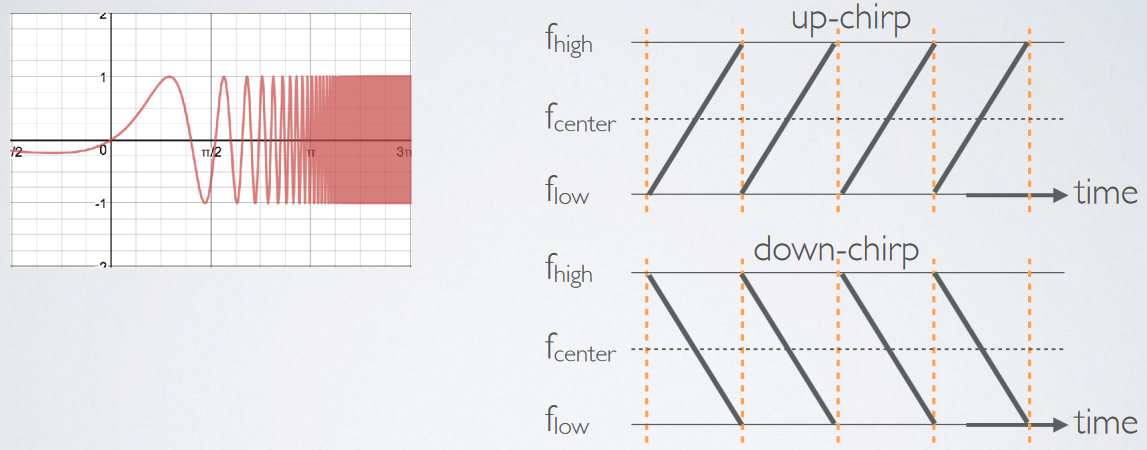
\includegraphics[width=0.9\textwidth]{pictures/chirp-sf}
 \caption[chirp spread spectrum]{chirp spread spectrum \cite{lora2022}}
 \label{fig:css}
\end{figure}

Die gleichmäßige Änderung der Frequenz innerhalb eines definierten Frequenzbereiches wird als chirp (zwitschern oder zirpen) bezeichnet und ist in der Natur weit verbreitet. So kommunizieren z.B. Vögel, Fledermäuse oder Delphine ebenfalls über die zeitliche Änderung der Frequenz. Dies hat den Vorteil, dass äußere Störungen einen geringeren Einfluss auf die Signalqualität ausüben und somit das Signal-Rausch-Verhältnis sich verbessert. Außerdem ist das CSS Verfahren weniger anfällig gegenüber den sogenannten Doppler-Effekt, bei dem es zu Signalverzerrungen bei dem Empfänger, wenn der Sender oder Empfänger in Bewegung sind, kommt. 

Durch das hinzufügen eines sogenannten Spreizfaktors (Spreading Factor oder SF), kann außerdem die Geschwindigkeit der zeitlichen Änderung der Frequenz, also die Chirprate geändert und damit auch die Datenrate variiert werden. LoRa definiert dabei insgesamt sechs Abstufungen des Spreizfaktors (SF6 bis inkl. SF12) \cite{sf2022}.

Grundsätzlich gilt; je kleiner der Spreizfaktor, desto höher ist die Chirprate und damit auch die Datenrate der Übertragung. Jedoch nimmt die Reichweite der Datenübertragung, je kleiner der Spreizfaktor ist, ab. Bei der Erhöhung des Spreizfaktors um einen Wert, halbiert sich die Chirprate und damit auch die Datenrate, aber die Reichweite wird erhöht. 

Auf der anderen Seite nimmt die Batterielaufzeit mit abnehmenden Spreizfaktor zu, da die Zeit, bei der das LoRa-Funkmodul zur Übertragung der Daten aktiv sein muss, aufgrund der erhöhten Chirp- bzw. Datenrate, abnimmt. 

Darüberhinaus kann durch die Erhöhung der Kanalbandbreite, bei gleichbleibenden Spreizfaktor, ebenfalls eine Erhöhung der Datenrate bewirkt werden. 

Mit der Änderung des Spreizfaktors und damit auch der Datenrate, können „Datenstaus“ im Netzwerk aktiv reguliert werden \cite{sf2022}. 

\subsection{LoRaWAN} \label{LoRaWAN}

Da LoRa anfangs nur für die Bitübertragungsschicht definiert wurde, musste ein Mechanismus entwickelt werden, bei dem die LoRa-Endgeräte addressiert untereinander und mit den LoRa-Gateways kommunizieren können. Es wurde zunächst einmal das LoRaMAC-Protokoll für die Sicherungsschicht (MAC layer) definiert. Später wurde die LoRa-Alliance\footnote{https://lora-alliance.org/} gegründet, die es zu LoRa-\textbf{W}ide-\textbf{A}rea-\textbf{N}etwork (LoRaWAN) umbenannt hat \cite{semtech2020}.

LoRaWAN nutzt für die Kommunikation zwischen den LoRa-Endgeräten und LoRa-Gateways die Sterntopologie (siehe Abb. \ref{fig:lorawan-topology}).

\begin{figure}[h]
 \centering
 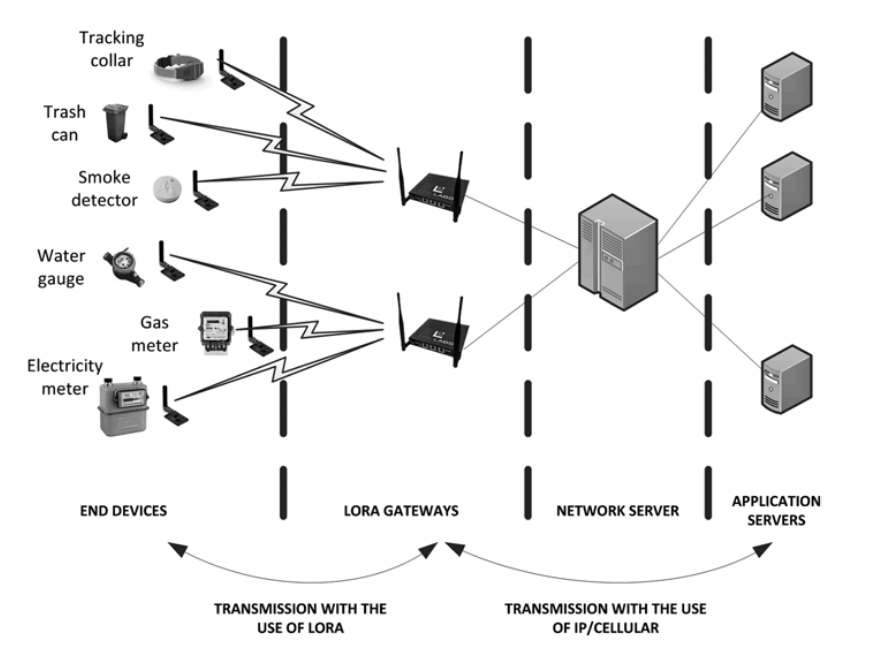
\includegraphics[width=0.9\textwidth]{pictures/lorawan-topology}
 \caption[LoRaWAN Topologie]{LoRaWAN Topologie \cite{Staniec2020}}
 \label{fig:lorawan-topology}
\end{figure}

Die LoRa-Endgeräte sammeln z.B. Sensor- und Messdaten und senden diese mithilfe von LoRa-Funktechnik an die LoRa-Gateways. 

Die LoRa-Gateways leiten die Daten dann über das Internet-Protokoll (IP), oder Mobilfunk an die Netzwerk-Server (Network Server) weiter. Es können mehrere LoRa-Gateways, die örtlich von einander getrennt sind, dazu genutzt werden, die Sensordaten der selben LoRa-Endgeräte zu empfangen. Durch die redundante Übertragung der selben Daten an mehrere Gateways, wird die Zuverlässigkeit und damit auch die Ausfallsicherheit der Datenübertragung verbessert.

Der Netzwerk-Server ist für die Entfernung der duplizierten Datenpakete, deren Dekodierung und für das Erstellen neuer Datenpakete, die an die LoRa-Endgeräte gesendet werden, zuständig. 

Schließlich verarbeiten die Anwendungs-Server (Application Server) die von den Netzwerk-Server erhaltene Daten für eigene Zwecke dann weiter. 


\section{MQTT} \label{MQTT}

\ldots


